We apply a data-driven method to estimate the $H \to \WW$ jet counting 
efficiency and its systematic uncertainties in data. 
In this method, the $H \to \WW$ jet counting efficiency in data $\epsilon_{H \to \WW}$
is estimated to be the value obtained from simulation multiplied by a data to simulation
scale factor from \dyll~events such that,

$$\epsilon_{H \to \WW} =  \epsilon_{H \to \WW} ({\epsilon_{\Z}^{data}}/{\epsilon_{\Z}^{MC}}).$$

The data to simulation correction factors are evaluated using the $Z$ events 
with dilepton mass around 7.5 GeV of the Z peak. 
Figure~\ref{fig:znjets} shows the number of Jets distributions, 
comparing data and MC for the Z events. A good agreement is seen. 
Figure~\ref{fig:jetveto_z} shows the leading jet $p_T$ spectrum and 
the jet-veto efficiency dependence on the leading jet $p_T$, comparing 
data and MC for the Z events. The data to simulation difference is within 1\%, 
much smaller than the theoretical uncertainties. 

We also study the dependence of the 0 and 1 Jet event fractions on the 
number of the pile up interactions, shown in Figure~\ref{fig:jetfrac_z}. 
With the chosen jet identification, the jet bin fraction has a very small
dependence on the number of pile up interactions, both in data and simulation. 

The uncertainty in $\epsilon_{H \to \WW}$ can be factorized into the 
$\Z$ efficiency uncertainty in data and the theoretical uncertainties in 
$H \to \WW/\Z$ efficiency ratio. 
The former is dominated by the statistical uncertainty. 
For the $H\to WW$ search, the theoretical uncertainties on the $H\to WW$ process are 
estimated by the LHC cross-section working group to be around 15\% for most of the higgs masses 
considered. More detail is discussed in Section~\ref{sec:systematics}. 
For the $\WW$ cross-section measurement the uncertainties on the $WW/Z$ efficiency ratio 
are estimated by varying the normalization and factorization scales in both 
MCFM and MC@NLO. The largest spead observed is assigned as the systematic uncertainties. 


%%%%%%%%%%%%%%%%%%%%%%%%%
\begin{figure}[!hbtp]
\centering
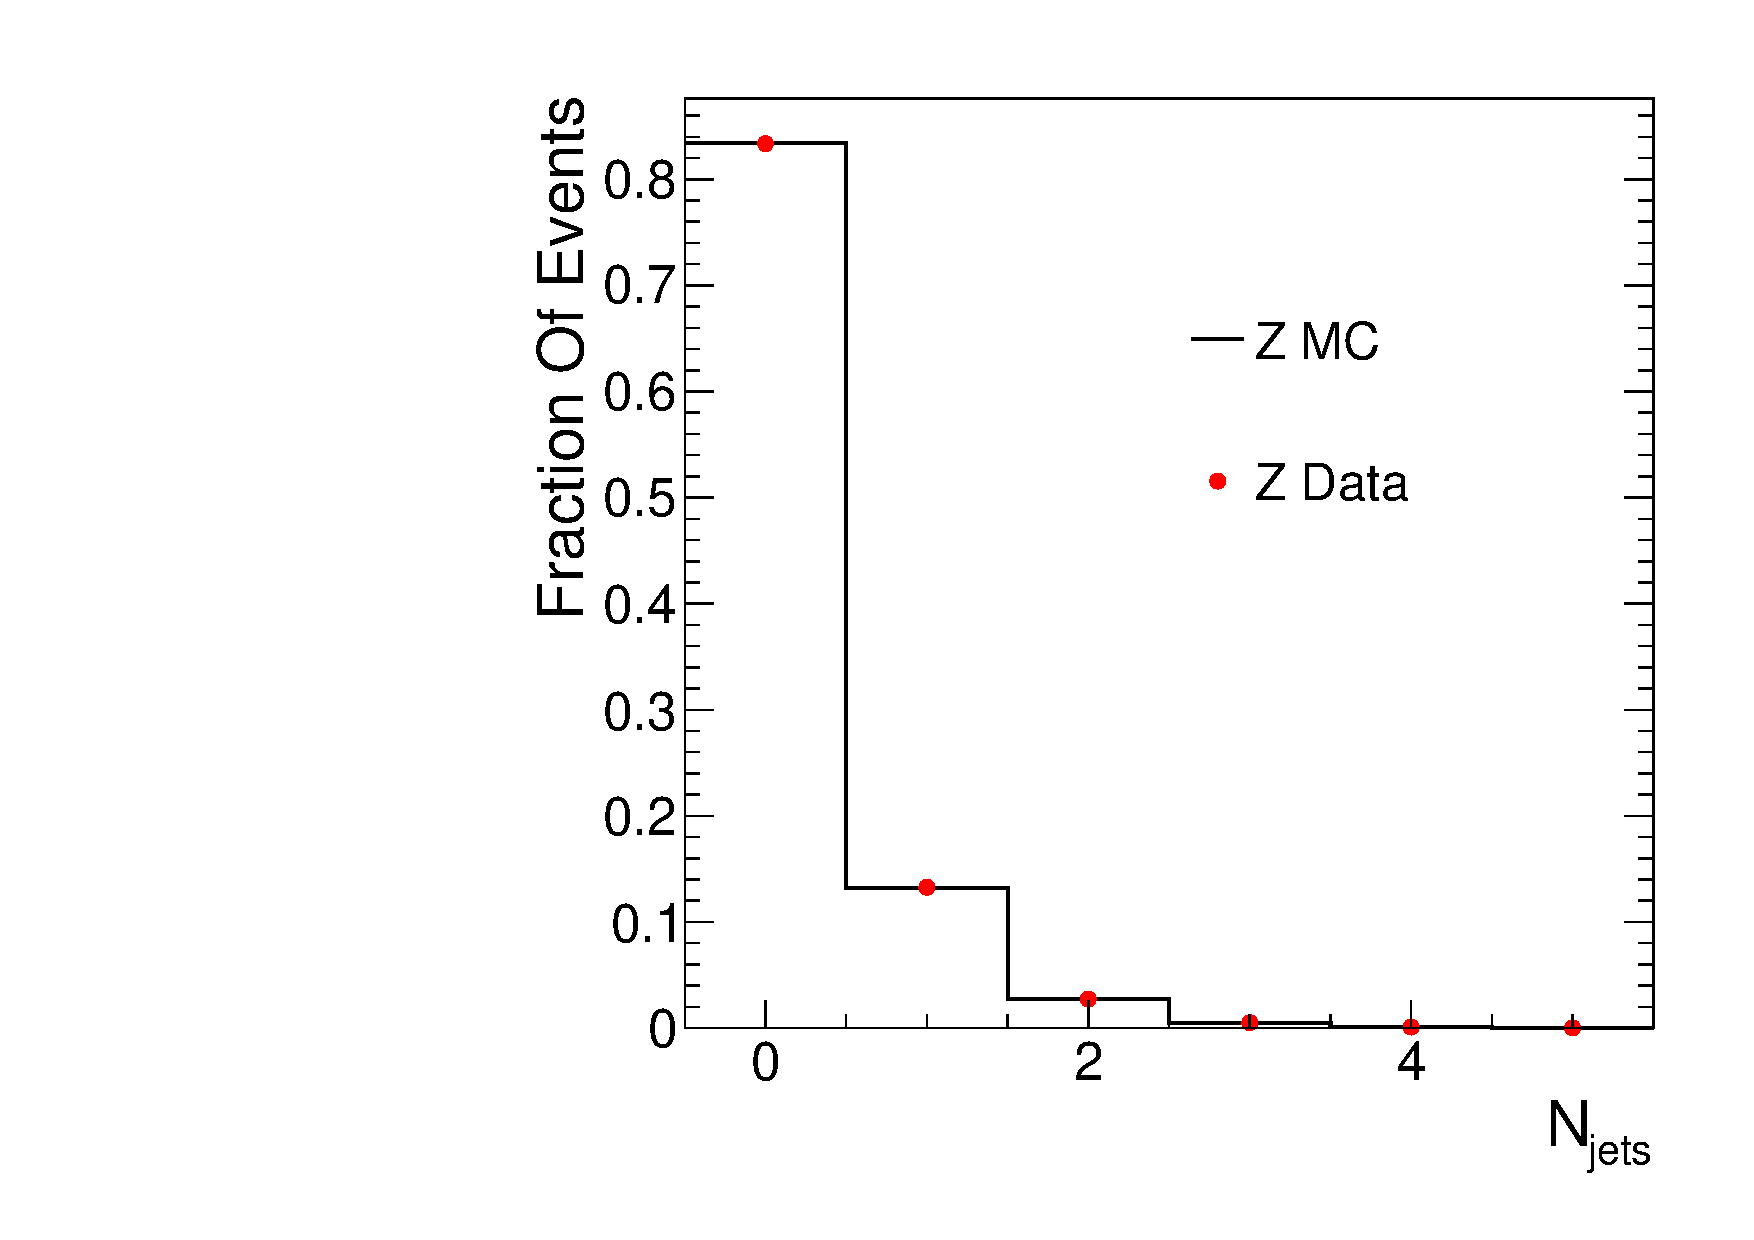
\includegraphics[width=.4\textwidth]{figures/Znjets.pdf}
\caption{The number of Jets observed in data (red solid dot) and MC (black line) for the Z events. }
\label{fig:znjets}
\end{figure}
%%%%%%%%%%%%%%%%%%%%%%%%%

%%%%%%%%%%%%%%%%%%%%%%%%%
\begin{figure}[!hbtp]
\centering
\subfigure[]{
\centering
\label{subfig:jetpt_z}
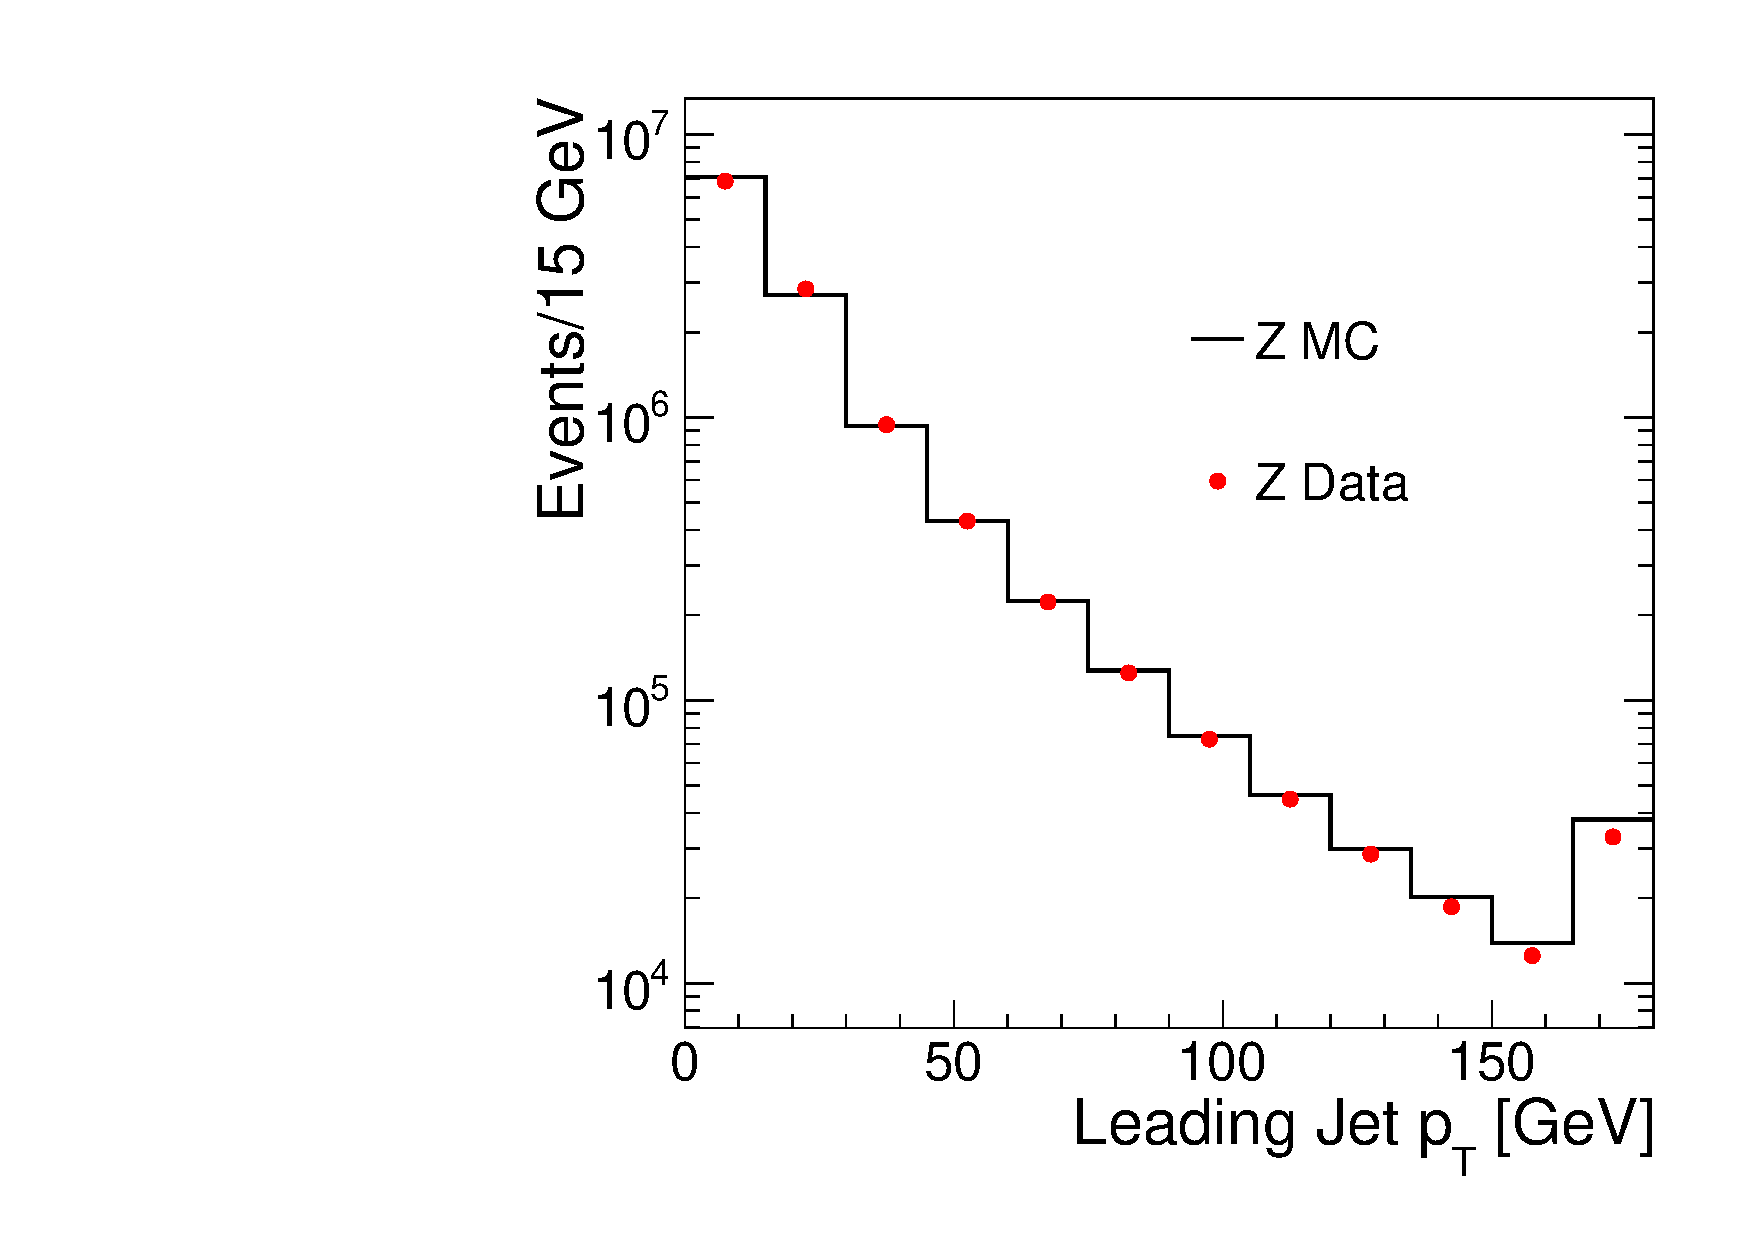
\includegraphics[width=.4\textwidth]{figures/ZjetpT.pdf}
}
\subfigure[]{
\centering
\label{subfig:jetveto_z}
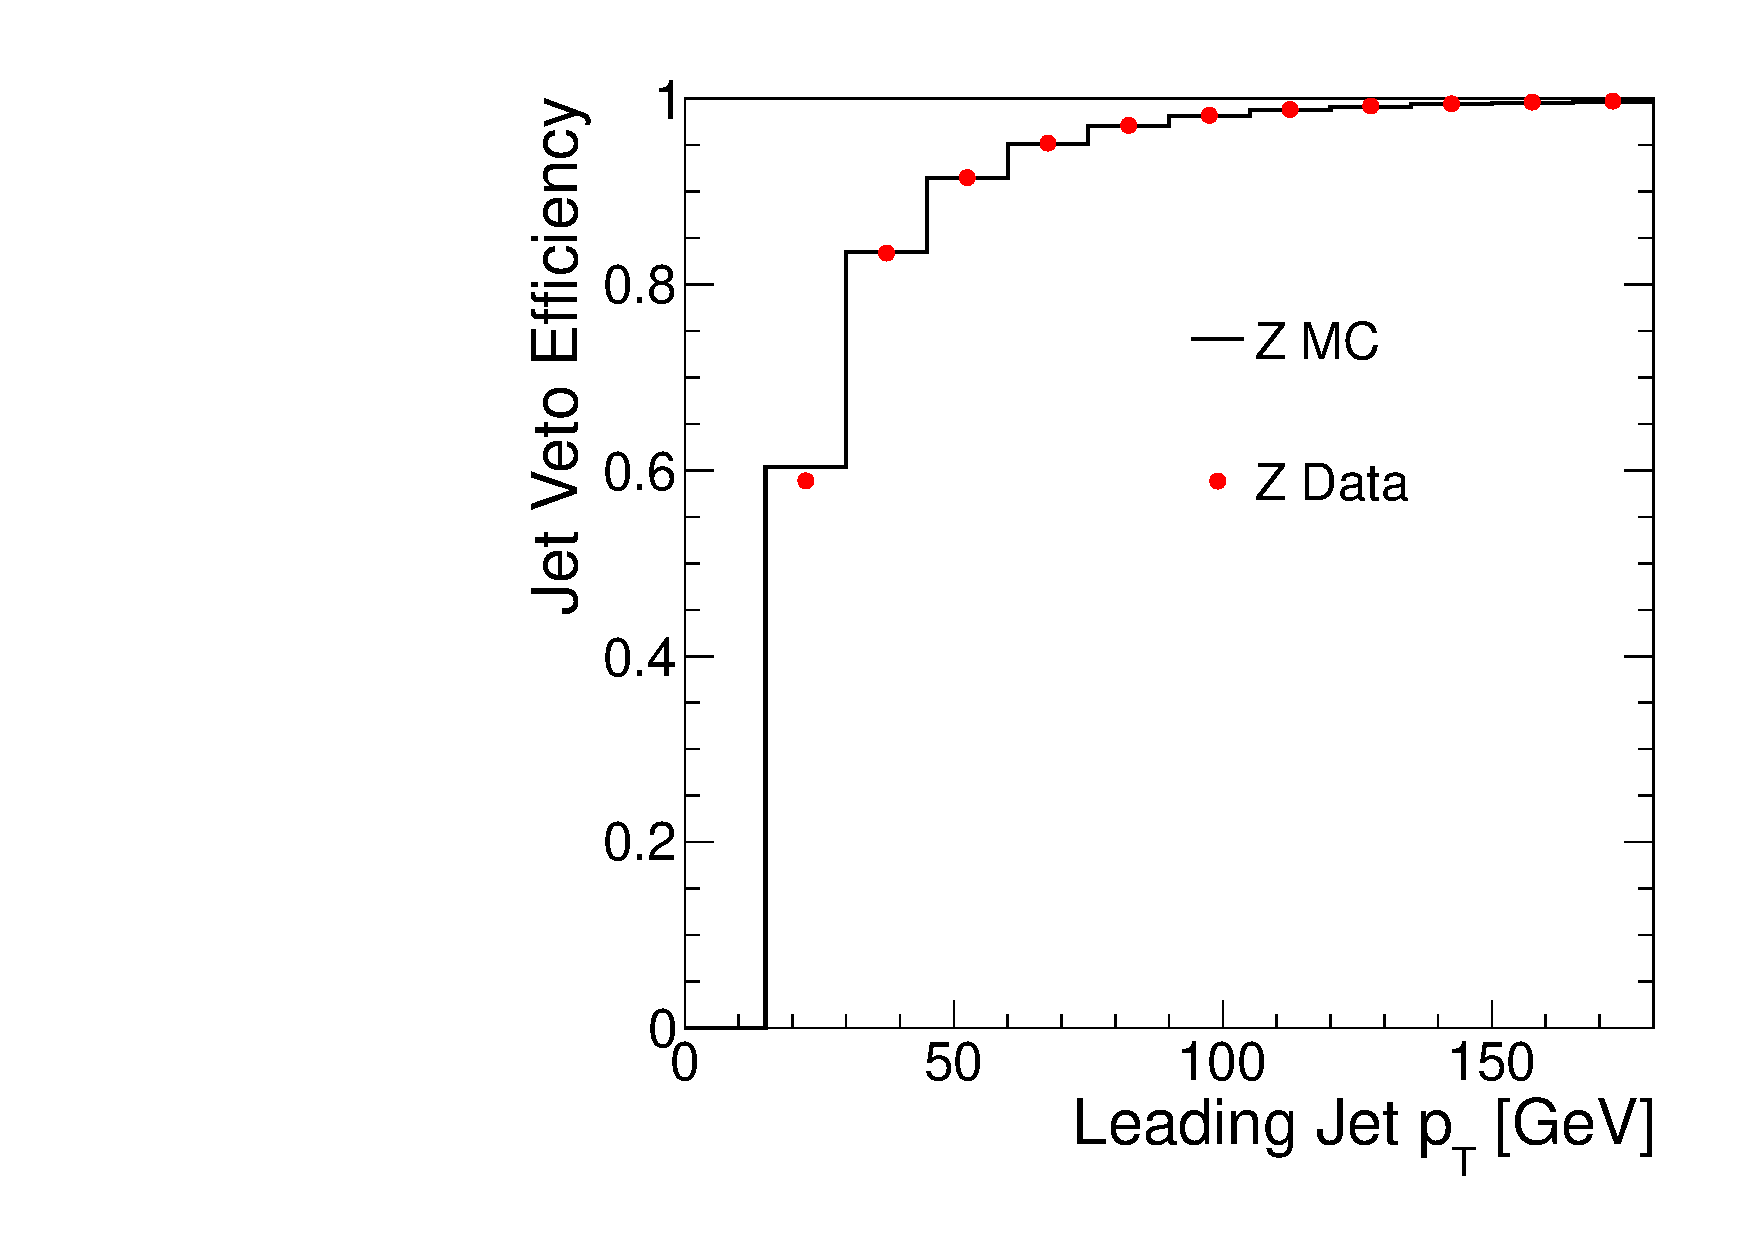
\includegraphics[width=.4\textwidth]{figures/Zjetvetoeff.pdf}
} \\
\caption{The leading jet $pT$ \subref{subfig:jetpt_z} and the jet veto efficiency as a function 
of the leading jet $p_T$ \subref{subfig:jetveto_z} in data (red solid dot) and MC (black line) for the Z events. }
\label{fig:jetveto_z}
\end{figure}
%%%%%%%%%%%%%%%%%%%%%%%%%

%%%%%%%%%%%%%%%%%%%%%%%%%
\begin{figure}[!hbtp]
\centering
\subfigure[]{
\centering
\label{subfig:zerojetfrac_z}
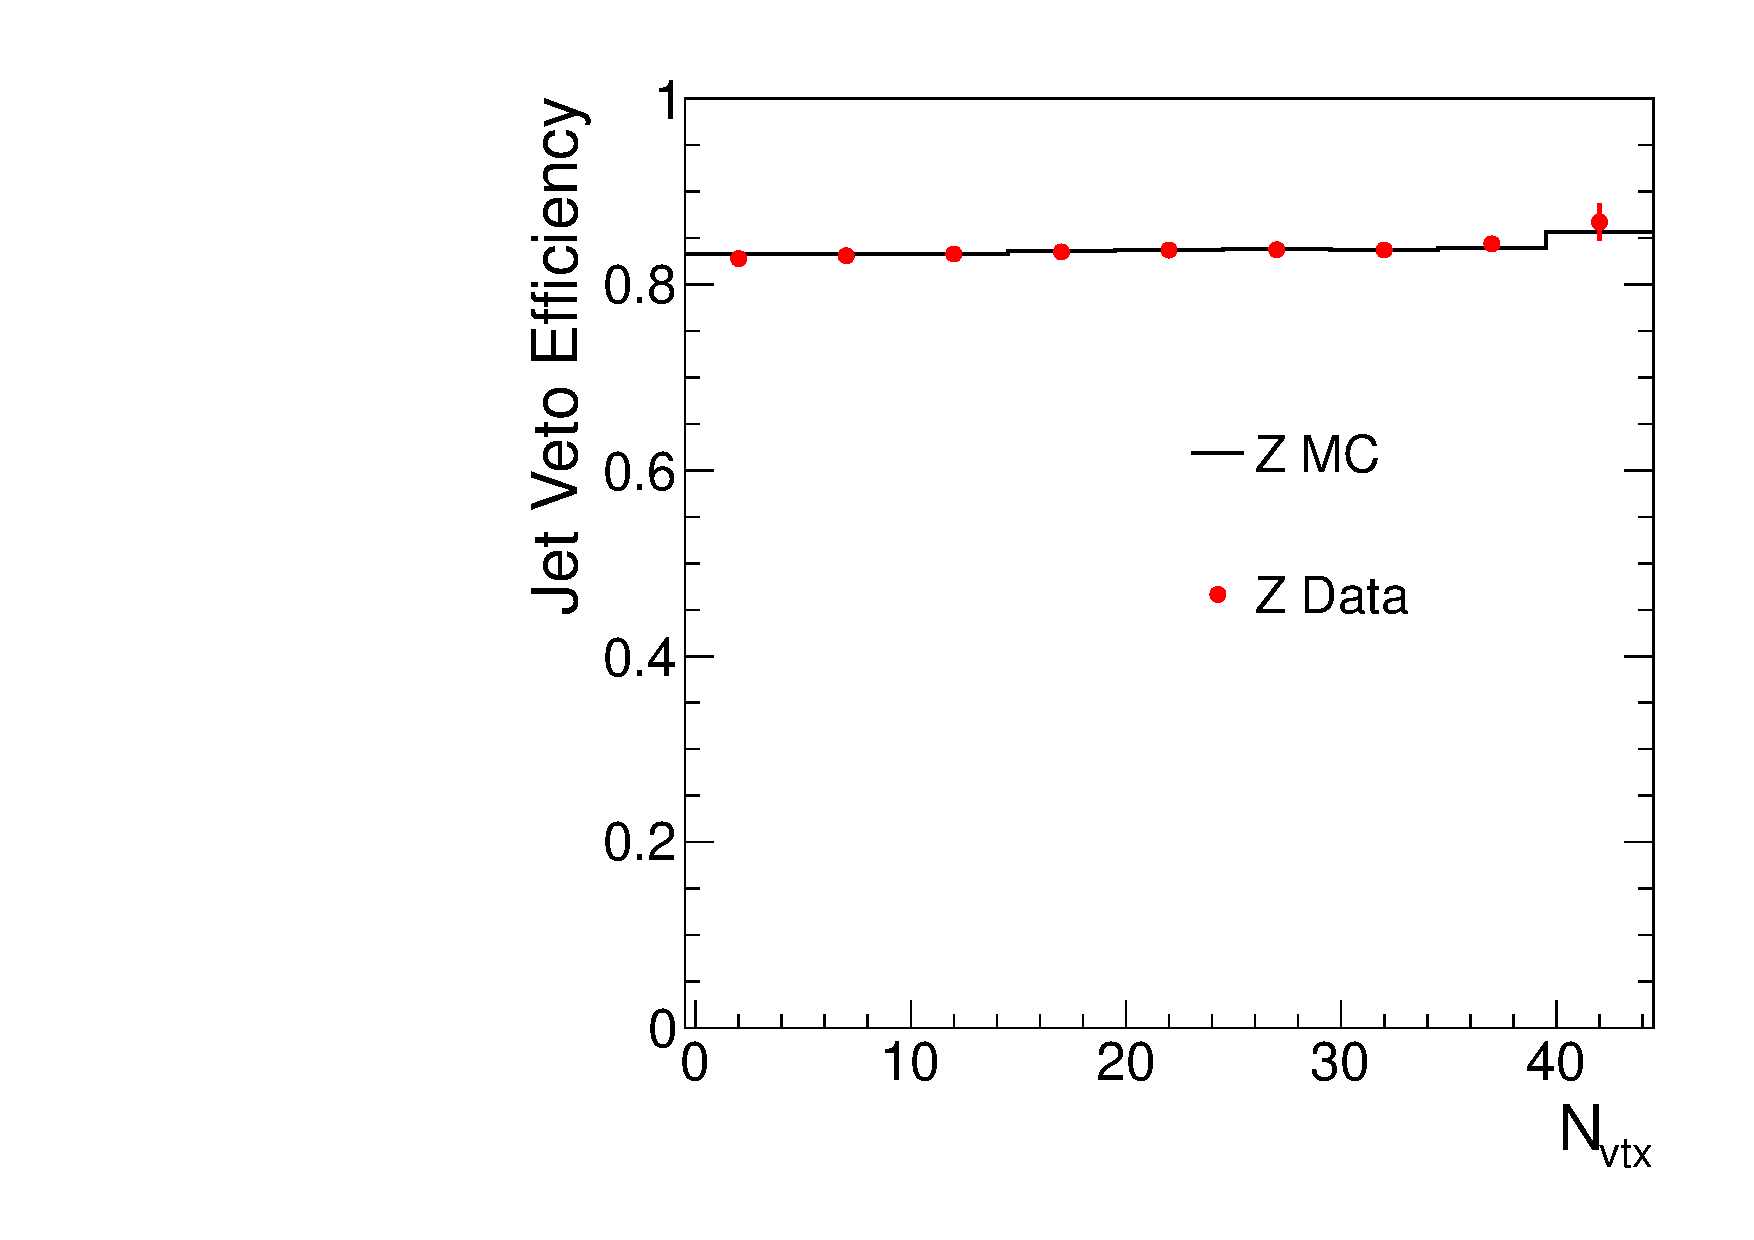
\includegraphics[width=.4\textwidth]{figures/Zjetvetoeff_vs_nvtx.pdf}
}
\subfigure[]{
\centering
\label{subfig:onejetfrac_z}
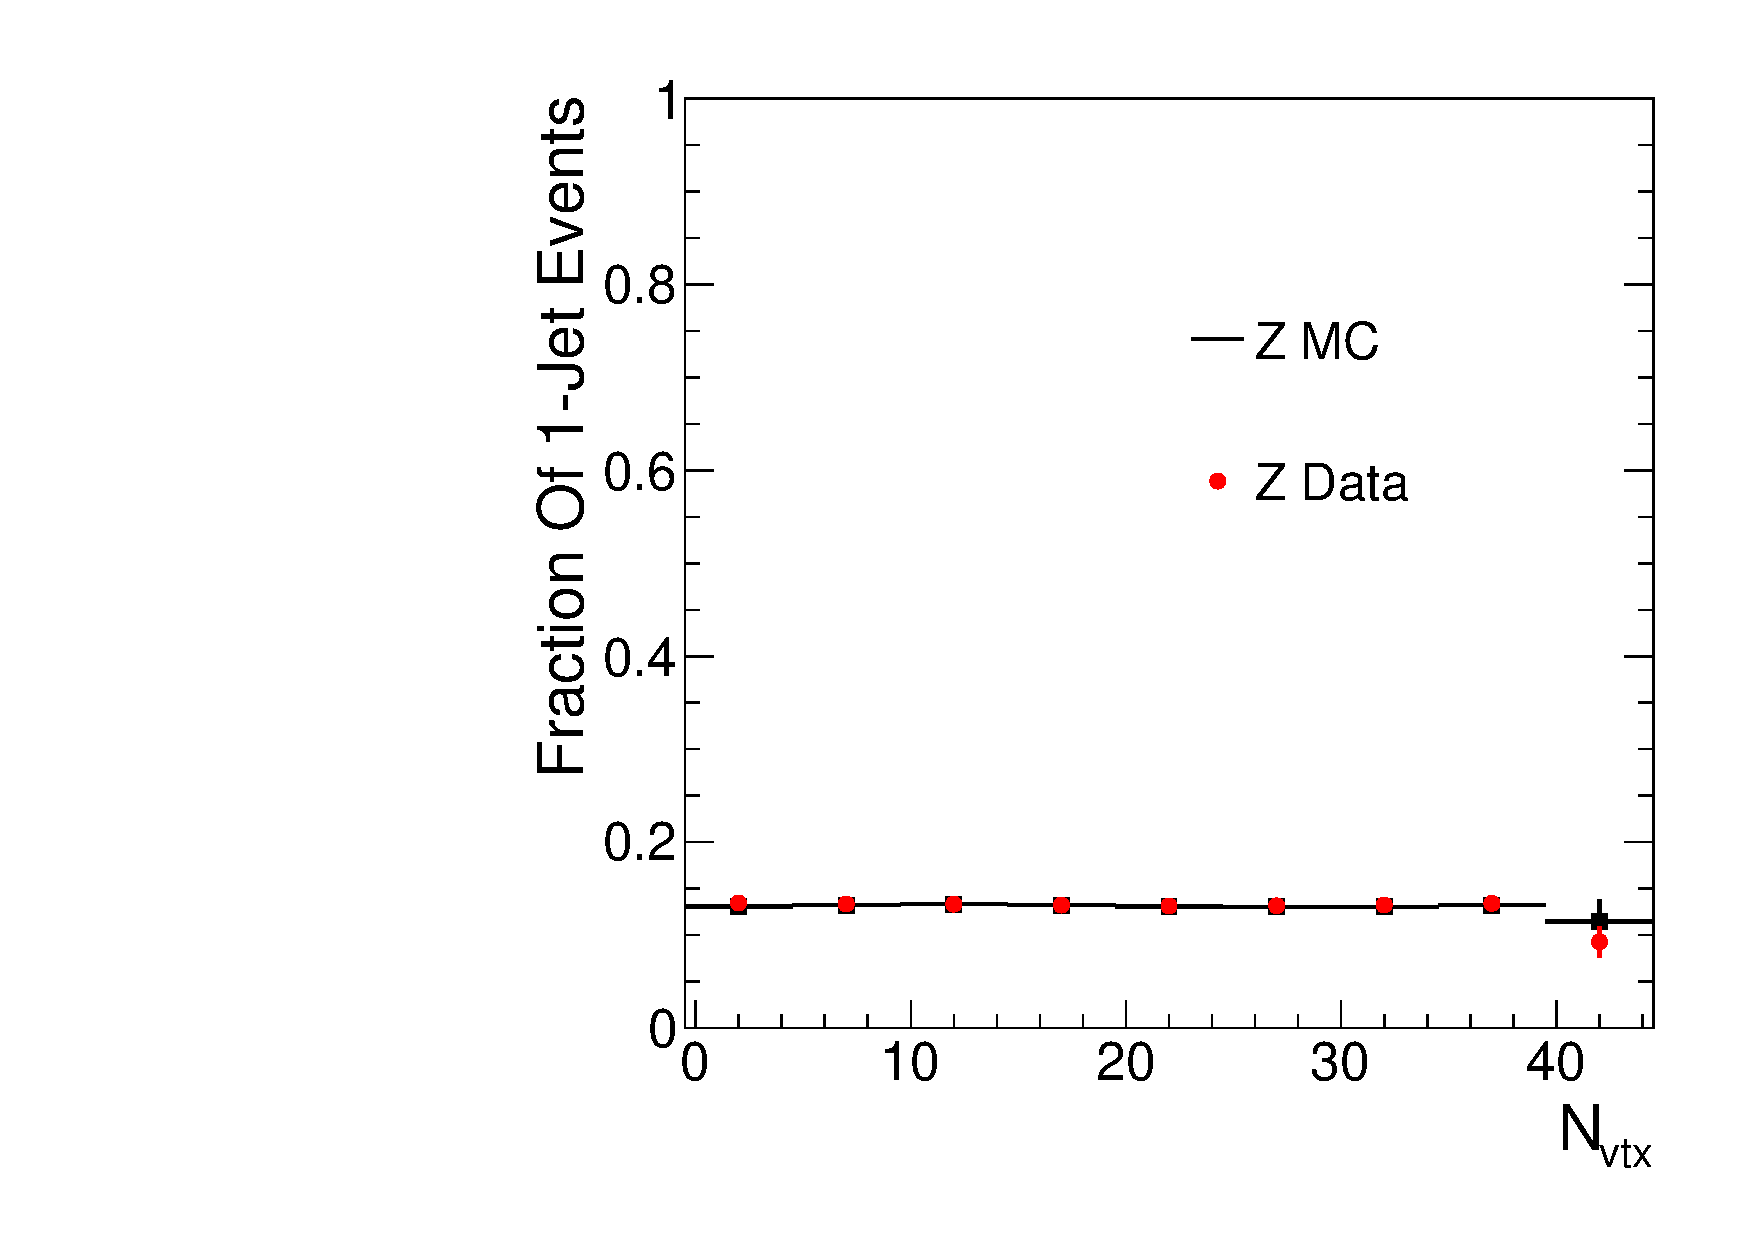
\includegraphics[width=.4\textwidth]{figures/Zonejeteff_vs_nvtx.pdf}
}\\
\caption{The fraction of events with 0 Jet \subref{subfig:zerojetfrac_z} and 1 Jet \subref{subfig:onejetfrac_z} 
as a function of the number of vertices, comparing data (red solid dot) and MC (black solid square) for the Z events. }
\label{fig:jetfrac_z}
\end{figure}
%%%%%%%%%%%%%%%%%%%%%%%%%



